%! Author = Len Washington III
%! Date = 10/30/24

% Preamble
\documentclass[
	date={November 6{,} 2024},
	month={11},
	day={6}
]{math486notes}
\usetikzlibrary{arrows.meta}

% Document
\begin{document}

\tableofcontents

\begin{equation*}
\begin{aligned}
	x = F(\tau, R_{0})
\end{aligned}
\end{equation*}
where $x = \frac{I}{N}$, $\tau = \mu t$, and $R_{0} = N\frac{\beta}{\mu}$

\begin{equation*}
\begin{aligned}
	\frac{dx}{d\tau} &= R_{0}(1-x)x - x\\
	&= R_{0}x - x^{2} - x\\
	&= x(R_{0} - 1 - x)\\
\end{aligned}
\end{equation*}

\begin{equation*}
\begin{aligned}
	\frac{ds}{dt} &= -\beta is\\
	\frac{di}{dt} &= \beta is - \mu i\\
\end{aligned}
\end{equation*}

\begin{equation*}
\begin{aligned}
	\frac{di}{dt} &= \beta is - \mu i\\
	\frac{di}{dt} &= i(\beta s - \mu)\\
	\frac{di}{i} &= (\beta s - \mu)dt\\
	\int \frac{di}{i} &= \int (\beta s - \mu)dt\\
	\ln |i| &= \beta st - \mu t + C\\
	i &= e^{\beta st - \mu t + C}\\
	  &= e^{\beta st - \mu t}e^{C}\\
	  &= Ae^{(\beta s - \mu) t}\\
\end{aligned}
\end{equation*}

\begin{equation*}
\begin{aligned}
	\frac{ds}{d\tau} &= -R_{0} is\\
	\frac{di}{d\tau} &= R_{0}is - i\\
\end{aligned}
\end{equation*}

Stability Analysis:
Locate nullclines:

\begin{equation*}
\begin{aligned}
	0 &= \frac{ds}{d\tau}\\
	&= -R_{0}is\\
	&= is\\
\end{aligned}
\end{equation*}
\begin{equation*}
\begin{aligned}
	s &= 0 \sep i &= 0\\
\end{aligned}
\end{equation*}
\begin{equation*}
\begin{aligned}
	0 &= \frac{di}{d\tau}\\
	&= R_{0}is - i\\
	&= i(R_{0}s - 1)\\
\end{aligned}
\end{equation*}
\begin{equation*}
\begin{aligned}
	i &= 0 \sep R_{0}s - 1 &= 0\\
	& \sep R_{0}s &= 1\\
	& \sep s &= \frac{1}{R_{0}}\\
\end{aligned}
\end{equation*}
Domain: $0 \leq s + i \leq 1$

If $R_{0} > 1$, the line will be inside the domain, else ($R_{0} < 1$), it is outside the domain.

If $R_{0} > 1$, the infection increases when $s > \frac{1}{R_{0}}$ and dies out when $s < \frac{1}{R_{0}}$.

If $R_{0} < 1$, then the rate of change of the infection dying out will be constant.

$s(t)$, $i(t)$ - set of parametric equations.
We want the equation of the parametric curve.

\begin{equation*}
\begin{aligned}
	\frac{ds}{d\tau} &= -R_{0}is\\
	\frac{di}{d\tau} &= R_{0}is - i\\
	\frac{di}{ds} &= \frac{di}{d\tau} \times \frac{d\tau}{ds}\\
	&= \frac{R_{0}is - i}{-R_{0}is}\\
	&= -\frac{R_{0}s - 1}{R_{0}s}\\
	&= -1 + \frac{1}{R_{0}s}\\
	&= -1 + \frac{1}{R_{0}} \frac{1}{s}\\
	\int \frac{di}{ds} &= \int \left( -1 + \frac{1}{R_{0}} \frac{1}{s} \right)\\
	\int di &= \int \left( -1 + \frac{1}{R_{0}} \frac{1}{s} \right) ds\\
	i &= -s + \frac{1}{R_{0}} \ln(s) + C\\
\end{aligned}
\end{equation*}
\begin{equation*}
\begin{aligned}
	\frac{ds}{di} &= \frac{ds}{d\tau} \times \frac{d\tau}{di}\\
	&= \frac{-R_{0}is}{R_{0}is - i}\\
	&= -\frac{R_{0}s}{R_{0}s - 1}\\
	&= \frac{R_{0}s}{1 - R_{0}s}\\
\end{aligned}
\end{equation*}

\section{Next COVID model (SIRS)}\label{sec:next-covid-model-(sirs)}

\begin{figure}[H]
	\centering
	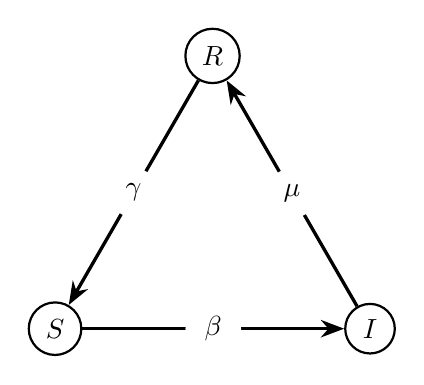
\begin{tikzpicture}[scale=2]
		\begin{scope}[every node/.style={circle,thick,draw}]
			\node (S) at (0,0) {$S$};
			\node (I) at (2,0) {$I$};
			\node (R) at (1,1.732) {$R$};
		\end{scope}
		\begin{scope}[>={Stealth[black]},
			every node/.style={fill=white,circle},
			every edge/.style={draw=black,very thick}]
			\path [->] (S) edge node {$\beta$} (I);
			\path [->] (I) edge node {$\mu$} (R);
			\path [->] (R) edge node {$\gamma$} (S);
		\end{scope}
	\end{tikzpicture}
	\caption{SIRS Model}
	\label{fig:sirs-model}
\end{figure}


Assume fraction: $s + i + r = 1$

\begin{equation*}
\begin{aligned}
	\frac{ds}{dt} &= -\beta si + \gamma r, \sep s(0) = s_{0} < 1\\
	\frac{di}{dt} &= \beta si - \mu i, \sep i(0) = i_{0} < 1\\
	\frac{dR}{dt} &= \mu i - \gamma r, \sep r(0) = 0
\end{aligned}
\end{equation*}


\end{document}